% This is based on the LLNCS.DEM the demonstration file of
% the LaTeX macro package from Springer-Verlag
% for Lecture Notes in Computer Science,
% version 2.4 for LaTeX2e as of 16. April 2010
%
% See http://www.springer.com/computer/lncs/lncs+authors?SGWID=0-40209-0-0-0
% for the full guidelines.
%
\documentclass{llncs}


\usepackage{graphicx}
\usepackage{placeins}
\usepackage{float}
\usepackage{subfigure}
\usepackage{multirow}
\usepackage{amssymb}
\usepackage{xcolor}
\usepackage{verbatim}

\newcommand{\rs}[1]{{\color{blue}#1}}

\begin{document}



\title{Automatic Conversion of Activity Diagrams into Flexible Smart-home Apps}
%
\titlerunning{Automatic Conversion of Activity Diagrams into Flexible Smart-home Apps}  % abbreviated title (for running head)
%                                     also used for the TOC unless
%                                     \toctitle is used
%
\author{Nipuni Perera\inst{1} \and Roopak Sinha\inst{1}
}%
\authorrunning{Perera and Sinha} % abbreviated author list (for running head)
%
%%%% list of authors for the TOC (use if author list has to be modified)
\tocauthor{Nipuni Perera and Roopak Sinha}
%
\institute{IT \& Software Engineering, Auckland University of Technology, New Zealand\\
\email{nipuni.perera@aut.ac.nz},
\email{roopak.sinha@aut.ac.nz}}

\maketitle              % typeset the title of the contribution

\begin{abstract}
Our homes are getting smarter, thanks to the larger variety of sensor and actuator devices that can be integrated to provide complex services.
However, a key technical challenge is writing complex smart-home applications that can automatically operate in different smart-homes and use any available devices dynamically. This issue becomes amplified when domain-experts, such as doctors, who are not proficient in software development, are tasked with designing these applications. 

In this paper, we identify UML Activity Diagrams as the most appropriate visual design model that can be used intuitively by domain-experts to design smart-home applications. Then, through comprehensive architecture design, we propose a complete \textit{automatic translation tool}, which provides a fully-featured UML Activity Diagram editor and the first compiler (to the best of our knowledge) to convert Activity Diagram designs into highly flexible code that can run in any smart-home system. 
Our evaluation of the automatic translation tool shows that it provides many necessary improvements in usability, bringing us a step closer to deploying apps designed by domain-experts into our smart-homes.




\keywords{smart-home, dynamic configurations, visual plans, automatic code generation}
\end{abstract}
%

\section{Introduction}

Smart homes are equipped with a myriad of sensor and actuator devices that can enable complex services to assist residents. Smart-home software, collectively called ``apps"~\cite{ALAA201748}, is now getting increasingly complex, thanks to increasing needs for customisation as well as the introduction of innovative and disruptive devices and IoT technologies.  Fig.~\ref{figure:SmartHome}  shows a typical smart home with sensors for light intensity, dust levels and motion, as well as actuators such as lighting, refrigerator, etc. These devices can be controlled by one or more apps to provide customised services and care for the residents. 

\begin{figure}[!h]
    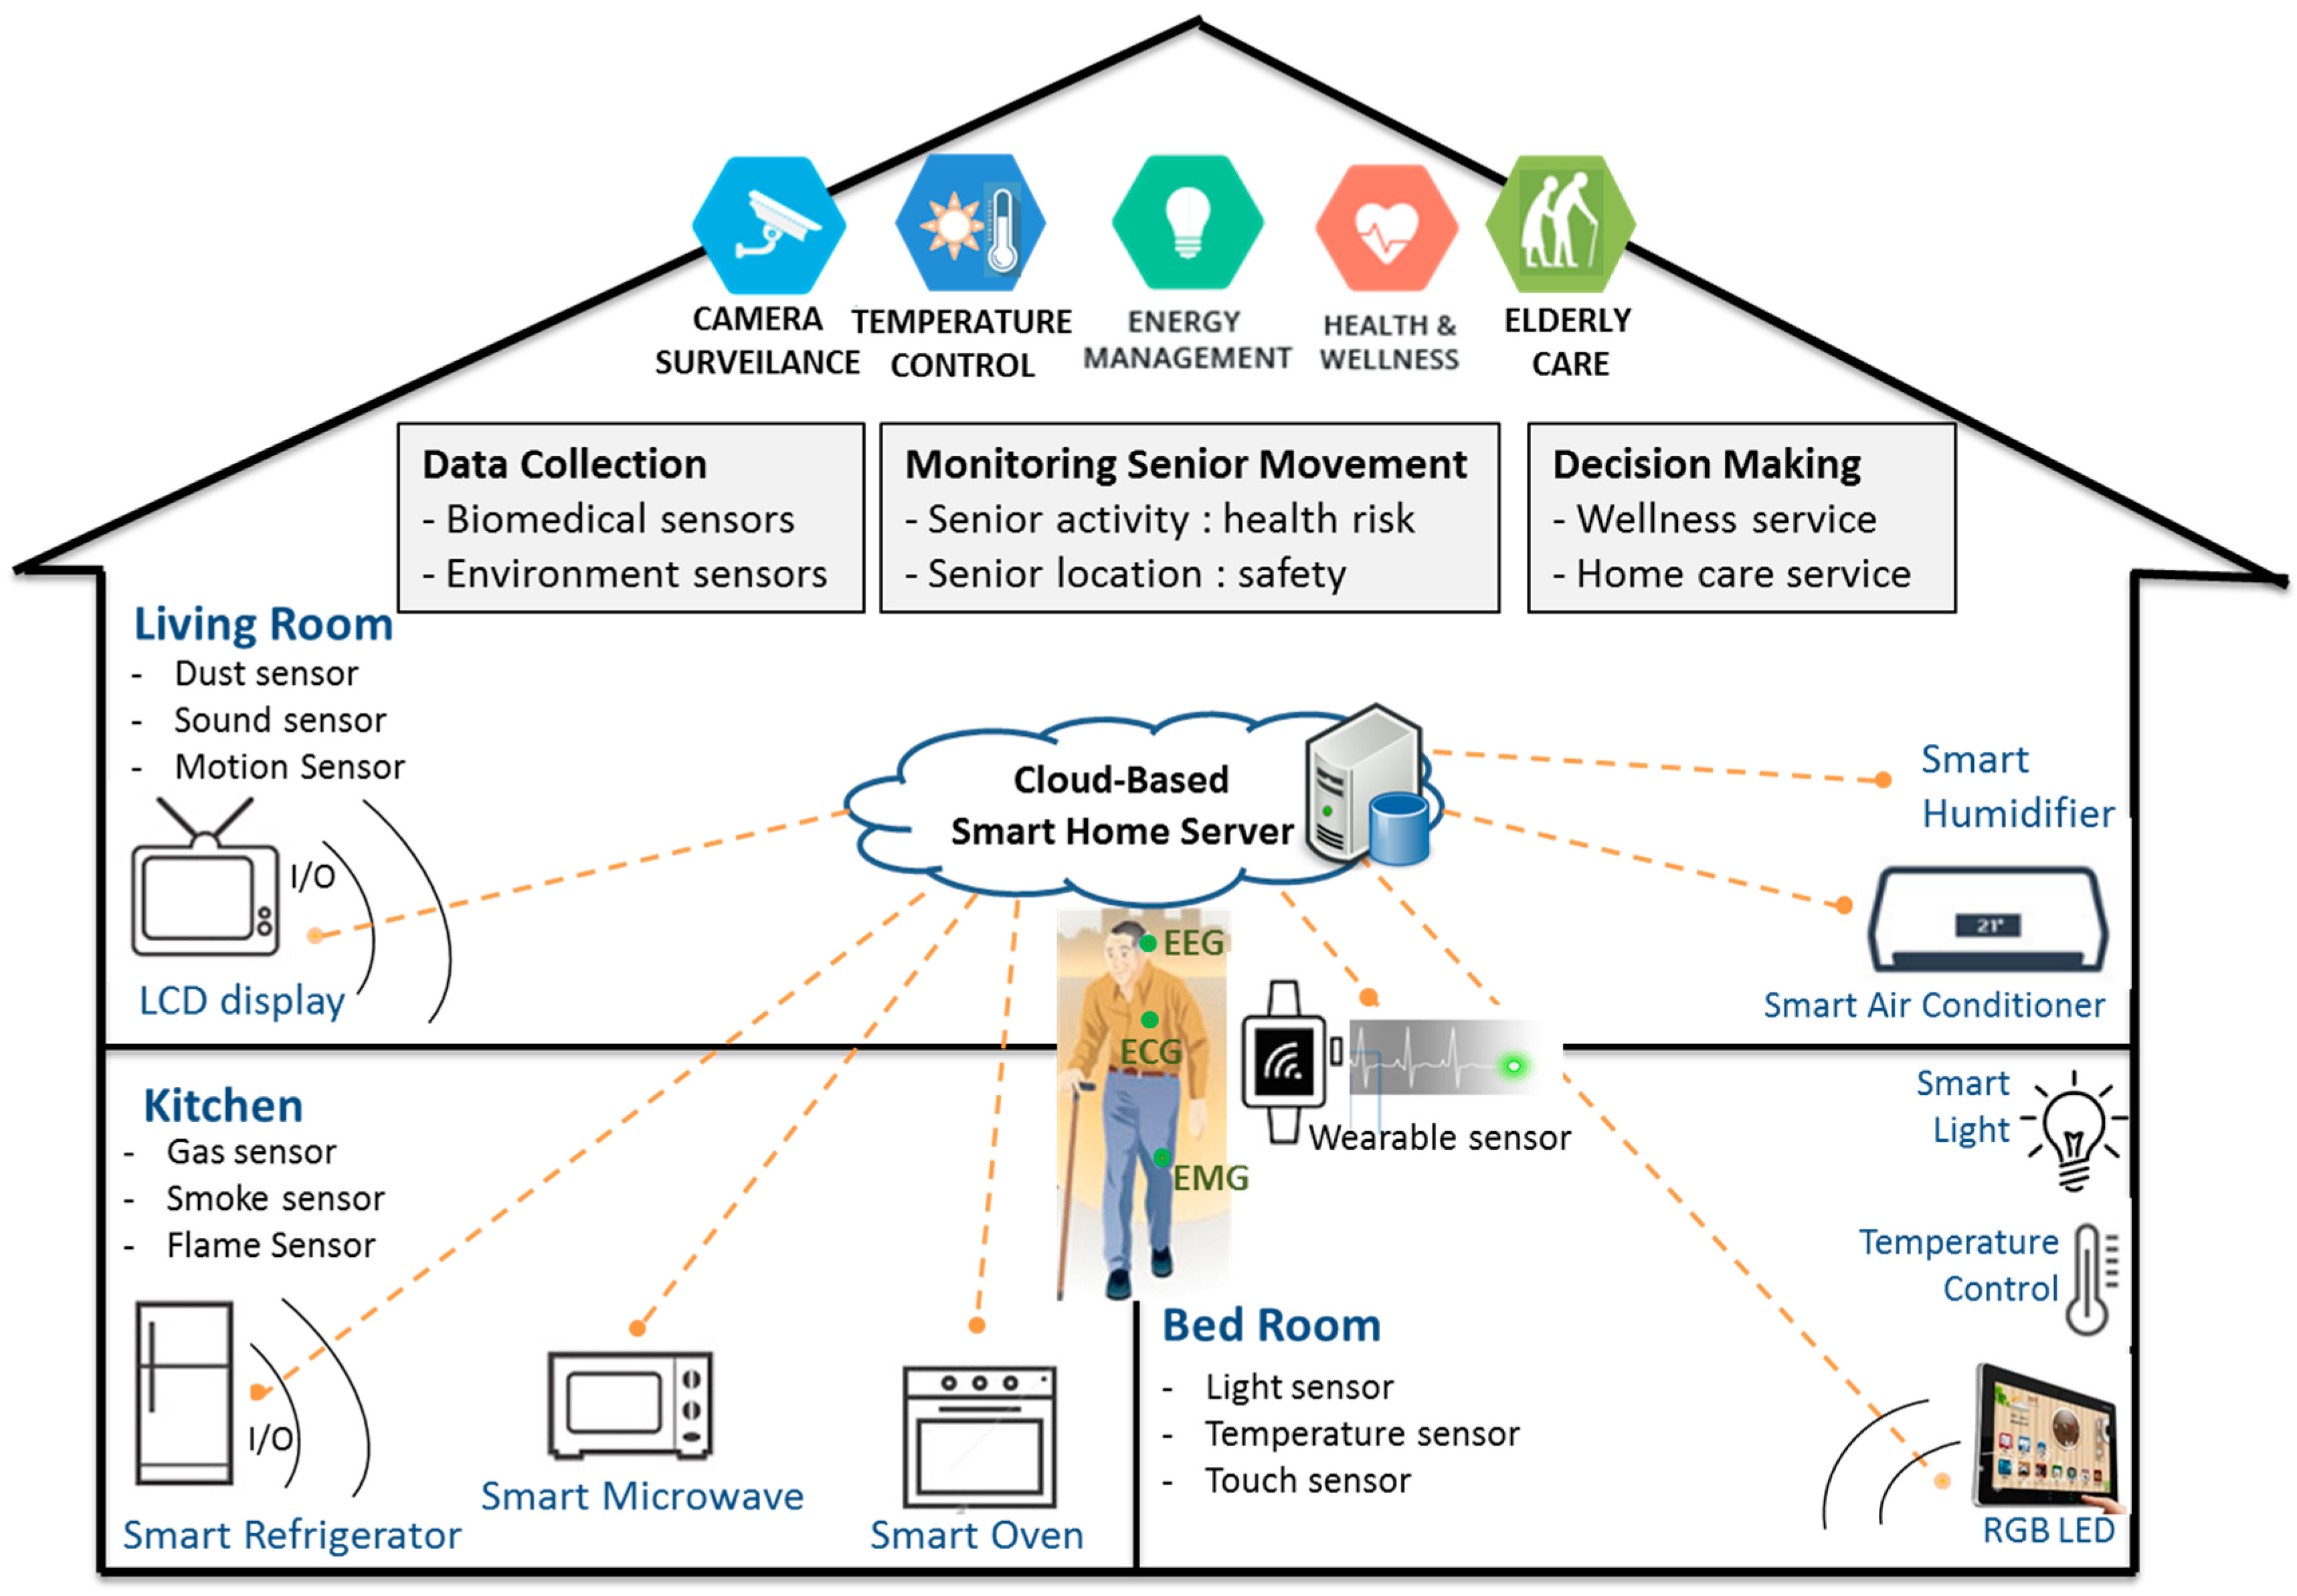
\includegraphics[width=\textwidth]{figs/smarthome}
    \caption{Smart Home \cite{jung2017hybrid}}
    \label{figure:SmartHome}
\end{figure}



There are a number of gaps in current research on designing smart home apps. 
These include a lack of interoperability between devices resulting in higher costs of deploying services~\cite{stojkoska2017review}, and implementing security measures such as confidentiality, integrity and availability~\cite{schneps2012wired}. Many current solutions target some of these problems, but often  fail to be effective in terms of usability which is a very important factor in the adoption of this technology. 

This paper focuses on the problem of easily creating and deploying smart-home apps. Existing tools or design models to create these apps cannot be readily used by non-experts, such as medical experts wanting to design apps for in-home care of their patients. Technically, the problem addressed in this paper is to efficiently and automatically generate correct code for these apps from \textit{behavioural} diagrams. Behavioral diagrams have been identified in this paper as more usable for non-experts wanting to design smart home apps (Sec.~\ref{sec:relatedworks}.
Also, existing automatic code-generators only work for \textit{structural} diagrams, such as UML Class Diagrams~\cite{rumpe2016modeling}.
This research addresses the following research questions:

\begin{enumerate}
\item \textbf{\textit{RQ1}} - Which factors lead to the choice of an app design model to address the challenges such as lack of interoperability between devices at the software level? 
\item \textbf{\textit{RQ2}} - What are the architectural characteristics of an automatic translation tool to convert an app design (based on the model developed after answering \textit{\textbf{RQ1}}) into a customized smart home app?
\item \textbf{\textit{RQ3}} - How can the high-level architecture of an automatic translation tool obtained from \textit{\textbf{RQ3}} lead towards the implementation of a prototype automatic translation tool?
\end{enumerate}




The design of this research followed a systematic literature review to refine and answer RQ1 and RQ2, and an adapted Design Science methodology to design and develop a solution to answer RQ3.
Fig.~\ref{figure:solution} shows an overview of the features of the solution, called the automatic translation tool. 
The tool automatically generates executable Java code from a UML Activity Diagram.
Activity Diagrams were identified as the most appropriate model for smart home apps while answering RQ1 (see Sec.~\ref{sec:relatedworks}).
The Eclipse-based automatic translation tool offers a fully featured editor for designing smart home apps.
The tool includes a compiler which accepts a visual plan, expressed as a UML activity diagram, and translates the visual plan into a runnable code which can then be deployed to a smart home application. 
An evaluation of the tool shows that the editor has high usability, and the compiler generates error-free and compact code, which can be deployed easily into any smart-home. 


%Pic1
\begin{figure}[!ht]
	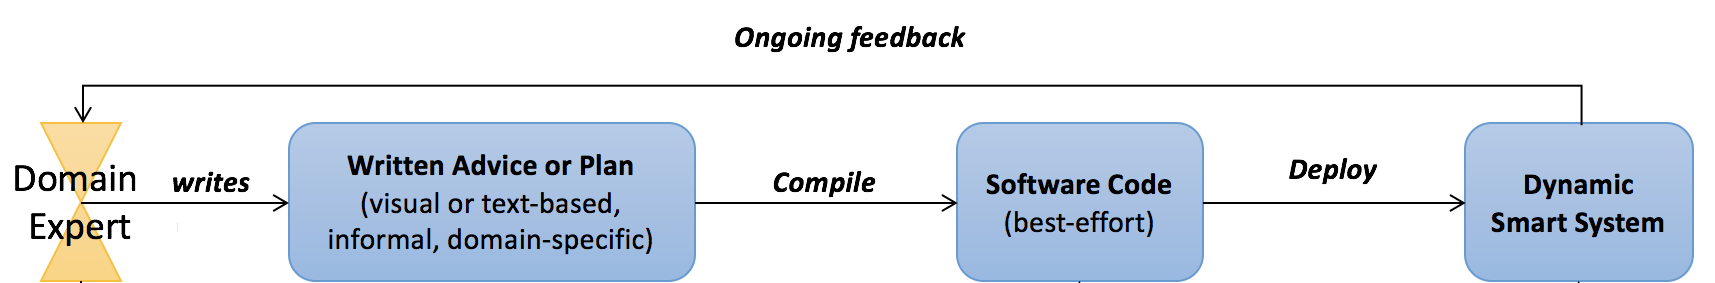
\includegraphics[width=\textwidth]{figs/Proposed_Solution}
	\caption{Overview of the automatic translation tool}
	\label{figure:solution}
\end{figure}


The primary contributions of this paper are:

\begin{enumerate}
\item \textbf{Choosing UML Activity Diagram as the more appropriate app design model for designing smart-home apps.} UML Activity diagrams are easier to use for non-experts due to their similarity with flowcharts, and also because they capture behavioral aspects rather than the structural aspects of a program. 

\item \textbf{User-friendly and fully-featured UML Activity Diagram Editor.} The editor features strong UML activity diagramming features, model element relationships and navigation among the model elements between the model editing space and the customized palette. Moreover, the editor can be used to design any smart home app. 

\item \textbf{Effective and Automatic Code Generation from Behavioral UML Activity Diagrams.} We have developed a compiler to generate correct executable Java code from UML activity diagrams that can be deployed in any smart home via a smart-phone.


\end{enumerate}







\section{Related Works}
\label{sec:relatedworks}

We conducted a systematic literature review to identify existing solutions for modelling smart-home software and candidate app design models for domain expert driven design of such apps. We also compare the surveyed works on key quality attributes like usability, interoperability, and customisability.
The details of this process are documented in~\cite{perera2018thesis}. This section presents the key findings from this comprehensive review.

\subsection{Current solutions for modelling smart-home applications}
%The existing solutions that answer the problem definition are categorized in to commercial and research based solutions. Each solution is addressed briefly below thus emphasizing their research gap. 

We identify two distinct classes of solutions - \textit{commercial} and \textit{research}. Commercial solutions are mature technologies that are available in the market today, while research solutions provide early proof-of-concept implementations only.

\noindent\textbf{Commercial solutions:} 
Solutions such as the Eclipse Smart Home (ESH) support both modelling and automatic code generation. 
The ESH framework, supported by the IoT platform~\cite{Smirek} provides modules for abstraction and translation functions thus enabling use cases and interaction across protocol boundaries. Even though this integrated system offers open personalized user interfaces based on a resource server, this may yet result in misuse and injection of malware, thus causing security and privacy issues \cite{Smirek}. 
AppleHealth offers an interactive solution to centralize mobile health applications and the management of health information. However, users need to have prior knowledge of web environments and gain familiarity with the provided web applications in order to take advantage of the services offered by these technologies~\cite{Vega-Barbas}. 
The SmartThings hub connects to motion sensors within a home and tracks anomalous activity. 
However, this framework has safety concerns, and can be misused by hackers for gaining access to a house~\cite{zillner2015white}. These solutions, as well as others like MisterHouse and Calos, provide very domain-specific capabilities that work only with compatible and mostly proprietary devices and software platforms.

 
\noindent\textbf{Research solutions}: 
The Simple Internet of Things (SITE)~\cite{Hafidh} initiative allows the users to specify and gain control of Internet of Things (IoT) smart objects. This solution supports modelling by end-users through a user interface or language for adding rules to control smart objects. However, this solution does not provide the ability to design more complex smart-home applications.
Parametric Statecharts and an associated compiler~\cite{sinha2017parametric} allow the visual modelling smart-home apps that may be deployed to smart-homes with different device configurations. These variances in configurations are captured as parameters in parametric Statechart designs, which are used to configure the application code at compile time. However, Statecharts are not easy to use for end users. Also, the inclusion of variables may simplify a design but this may cause difficulties during analysis\cite{stephan2013survey}.
Rule-based intelligence for domotic environments~\cite{Bonino}, targeted towards homes and hospitals, addresses two main challenges of lack of interoperability and insufficient support for advanced user-home interaction. Here, an Intelligent Domotic Environment (allows the integration of different automation systems, appliances, and devices into a single powerful environment, which is capable of providing Ambient Intelligence functionalities. However, this solution is unable to handle dynamicity and uncertainty in devices operating in smart environments. 

Tab~\ref{tab:compare} shows a comparison of the surveyed research and commercial solutions on key qualities of usability, interoperability and customizability. Usability is the degree to which the smart home user understands, uses, and adopts a solution~\cite{demiris2008findings}. Interoperability is the ability of a system to function with other systems without the need for need for special effort \cite{miller2000interoperability}. Customizability is the ability to customize an application based on user preferences \cite{groppe2005profile}.
Most solutions do not meet all these criteria. Often, the more usable solutions are proprietary and hence tightly coupled with the use of a small set of devices. 

%\subsection{Comparison of existing works}

\begin{table}[h!]
\footnotesize
    \begin{center}
        \begin{tabular}{|p{2cm}|p{3.5cm}|c|c|c|} \hline
        \textbf{Origin} & \textbf{Solution Name} & \multicolumn{3}{|c|}{\textbf{Comparison Criteria}}\\ \hline
        & &Usability & Interoperability &  Customizability \\ \hline
        \multirow{6}{*}{\textbf{Research}} & Simple IoT (SITE) & $\times$ & $\times$ & $\checkmark$ \\ \cline{2-5}
        & Parametric State Charts& $\times$ & $\checkmark$&  $\checkmark$ \\\cline{2-5}
        & Proactive Architecture& $\times$& $\checkmark$ &  N/A \\\cline{2-5}
        & Rule Based Intelligence& $\times$& $\checkmark$ &  N/A \\\cline{2-5}
        &Architecture for SDSM& $\checkmark$& $\checkmark$&  $\checkmark$ \\\cline{2-5}
        &Ontology System& $\times$ &$\times$&  N/A \\
        \hline
        \multirow{6}{*}{\textbf{Commercial}}& Eclipse Smart Home& $\times$& $\checkmark$&  $\checkmark$ \\\cline{2-5}
        &AppleHealth & $\times$ & N/A&  $\checkmark$ \\\cline{2-5}
        &SmartThings &  $\times$&$\checkmark$ &  $\checkmark$ \\\cline{2-5}
        &Ubiq Scenario Control& $\times$ &$\checkmark$ &  $\times$\\\cline{2-5}
        &MisterHouse& $\times$ &$\checkmark$ &  N/A\\\cline{2-5}
        &Calos&$\times$ &$\checkmark$ &  N/A\\
        \hline
        \end{tabular}
    \end{center}
    \caption{Comparison of Existing Solutions}
    \label{tab:compare}
\end{table}

\subsection{Selection of a suitable App design model}

As Tab.~\ref{tab:compare} shows, existing solutions fail to meet at least some of the desired qualities. This led us to analyse visual design models that are well-known or standardised, easy to use for non-experts, amenable to code generation, able to model smart home apps that integrate many sensor and actuator devices, etc. Tab.~\ref{tab:diagrams} shows the overall comparison of UML diagrams on these factors. UML was chosen as it is a standard design framework which also has a high availability of tools supporting its various diagrams. UML Activity diagrams featured the maximum number of desired qualities. Hence, this research then focussed on both customising UML Activity Diagrams for designing smart-home apps and to enable automatic code generation from such designs. Being a behavioural diagram type, no current compiler supports automatic code generation from UML Activity Diagrams.



\begin{table}[!h]
\footnotesize
    \begin{center}
        \begin{tabular}{ |p{4cm}|c|c|c|c|  } \hline
            
            Factors  & Class & Sequence & Activity & StateChart \\ \hline
            
            Quality Improvements & $\checkmark$   & $\checkmark$    & $\checkmark$    & $\checkmark$      \\ \hline
            Automated Code generation  & $\checkmark$    & $\checkmark$    & $\checkmark$    & $\checkmark$     \\ \hline
            Improved problem solving  & $\checkmark$    & $\checkmark$    & $\checkmark$    & $\checkmark$         \\    \hline
            Improved levels of usability  &  &  &  &  $\checkmark$     \\
            \hline
            Traceability & $\checkmark$    & $\checkmark$    & $\checkmark$    & $\checkmark$      \\ \hline
            Software architecture design activities  & $\checkmark$ &  & $\checkmark$    &     \\ \hline
            Task performance  & $\checkmark$  &  & $\checkmark$  &   \\ \hline
            Backlog control  &  &  &  &       \\    \hline
            Architectural analysis, synthesis and evaluation  &  &  &  &   \\    \hline
            Behavioral modelling &  &  &  & $\checkmark$   \\
            \hline
            Representation of the control flow of the system &  &  & $\checkmark$  &     \\
            \hline
            Specification of which object is responsible for which activity &  &  & $\checkmark$  &    \\
            \hline
            Software maintenance, modularity and re usability &  &  &  & $\checkmark$   \\
            \hline
            
            
            
            
            
            
            
        \end{tabular}
    \end{center}
    \caption{Evaluation and Selection of App Design Models}
    \label{tab:diagrams}
\end{table}
\section{Architecture Design}
\label{Architecture Design}

We followed Attribute-Driven Design (ADD)~\cite{clements2002documenting} to carry out the systematic creation of the architecture for our solution  based on the following key architectural drivers which include functional and Quality Attribute (QA) requirements:

\begin{enumerate}
    \item \textbf{Primary functional requirement}: the ability to generate code automatically from a visual design, which should accurately represent the intended behaviour.
    \item \textbf{QA1: Usability:} the solution should be as easy to use as possible.
    \item \textbf{QA2: Interoperability:} The solution should support the modelling of any correct design, which should be able to control a dynamic set of sensor and actuator devices.
   \item \textbf{QA3: Modularity:} The process of converting designs into code should be as modular as possible, so that we can use different transformation types to generate a variety of code in the future.
\end{enumerate}

The architectural drivers are used as the inputs to the architecture design process. This process involves several steps including the identification of architectural patterns and tactics, and documenting is using appropriate views. For our solution, the primary functional and quality attribute requirements are covered by two views: the logical view and the process view. These are described in the following subsections. 


\subsection{Logical view}

The logical view of our solution is presented as a class diagram in Fig.~\ref{fig:class}.
The logical view shows how a code base is structured to satisfy important architectural drivers.
It depicts how the functional requirements are achieved using successive model-to-model transformations of a given Activity Diagram Model into Java code.
These transformations are described in more detail in the next section.
The design of the Automatic Translation Tool is emphasized with the support of associations and compositions, which show how the primary functional requirement, as well as the desired quality of modularity.

\begin{figure}[!ht]
	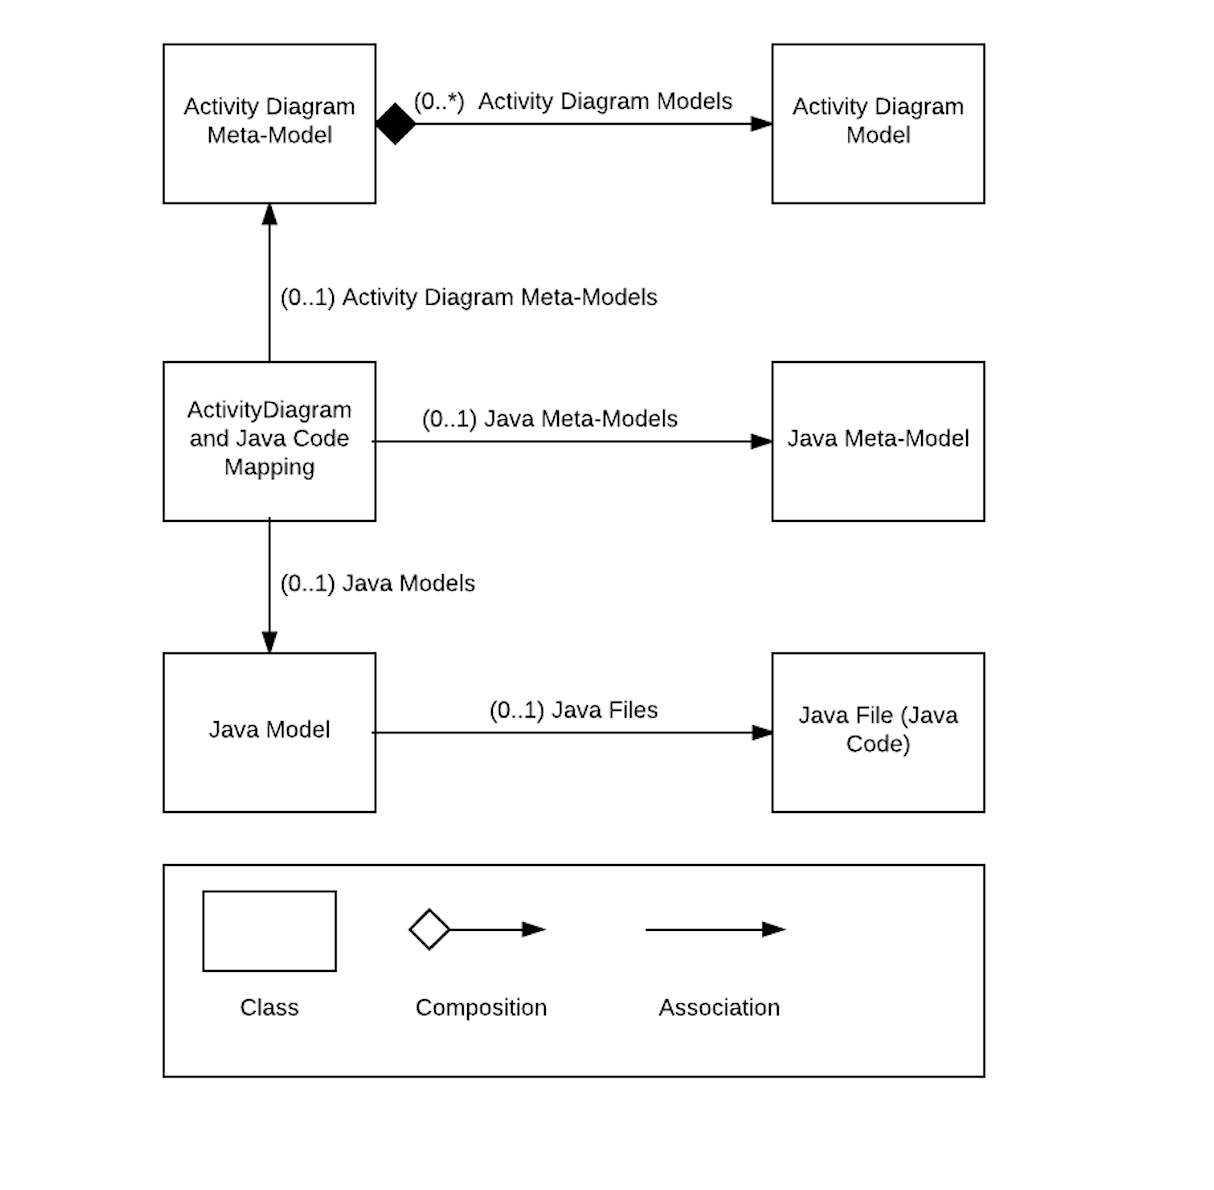
\includegraphics[width=\textwidth]{figs/Logical_View}
	\caption{UML Class Diagram: Automatic Translation Tool}
	\label{fig:class}
\end{figure}





\subsection{Process view}
The process view shows the dynamic aspects of the system and details the system processes and how the communication between various elements and entities are carried out when the system is operationalized~\cite{kruchten19954+}. The Activity Diagram shown in Fig.~\ref{figure:process} depicts the overall workflow of the tool's usage and ability to generate code in possibly different formats. The process view contributes to the key quality attributes of usability and interoperability.  

\begin{figure}[!h]
	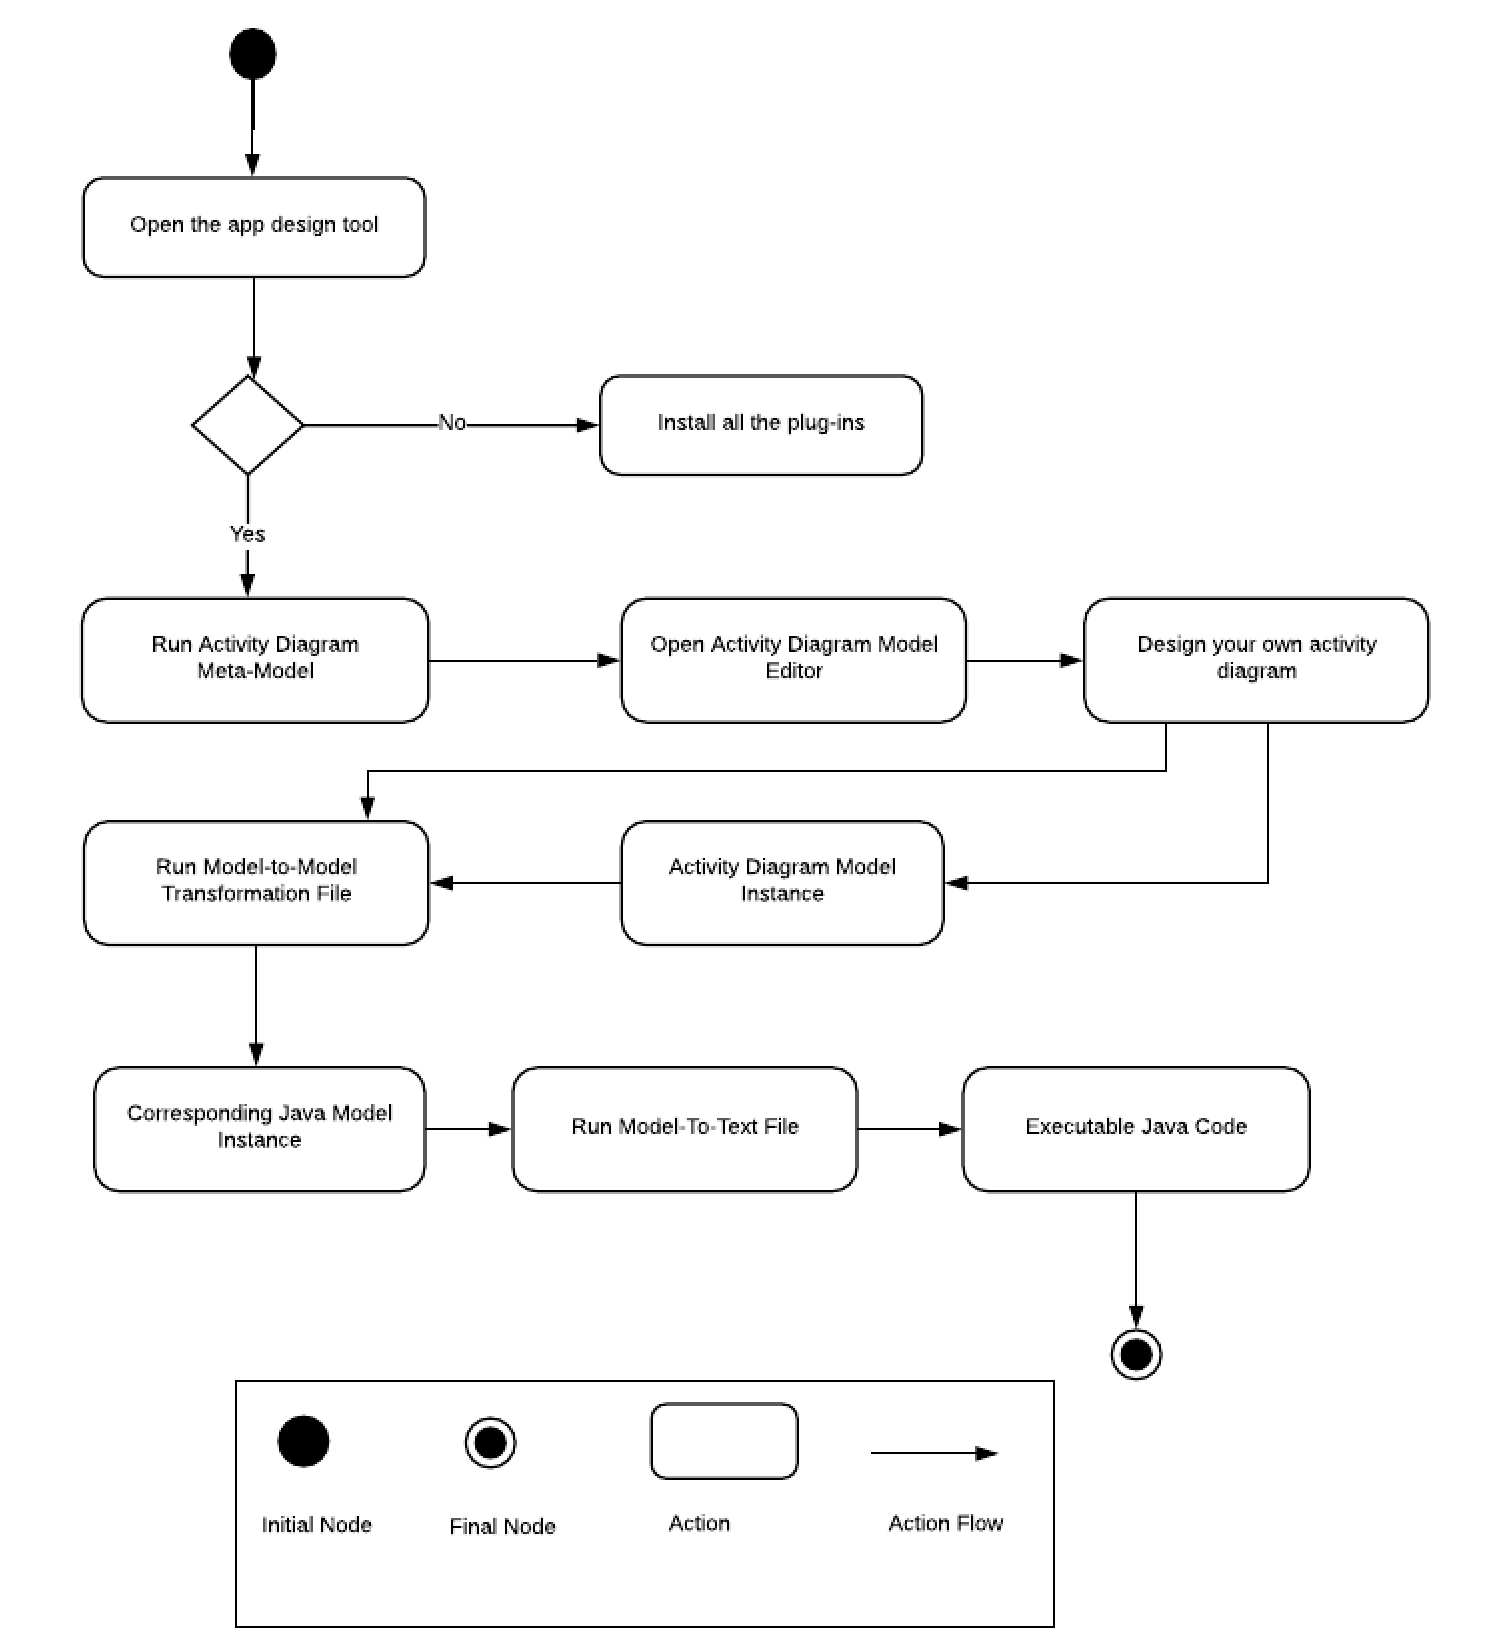
\includegraphics[width=\textwidth]{figs/ProcessView} 
	\caption{Process View}
	\label{figure:process}
\end{figure}




\section{Tool Development}
\label{Development}

The Automatic Translation tool comprises of a set of components such as the meta-models for UML Activity Diagram and Java, the Activity Diagram model editor, model to model transformations and model to text transformations. Each of these components is addressed in detail in this section, and is illustrated in Fig.~\ref{figure:overalltool}.

\begin{figure}[!h]
	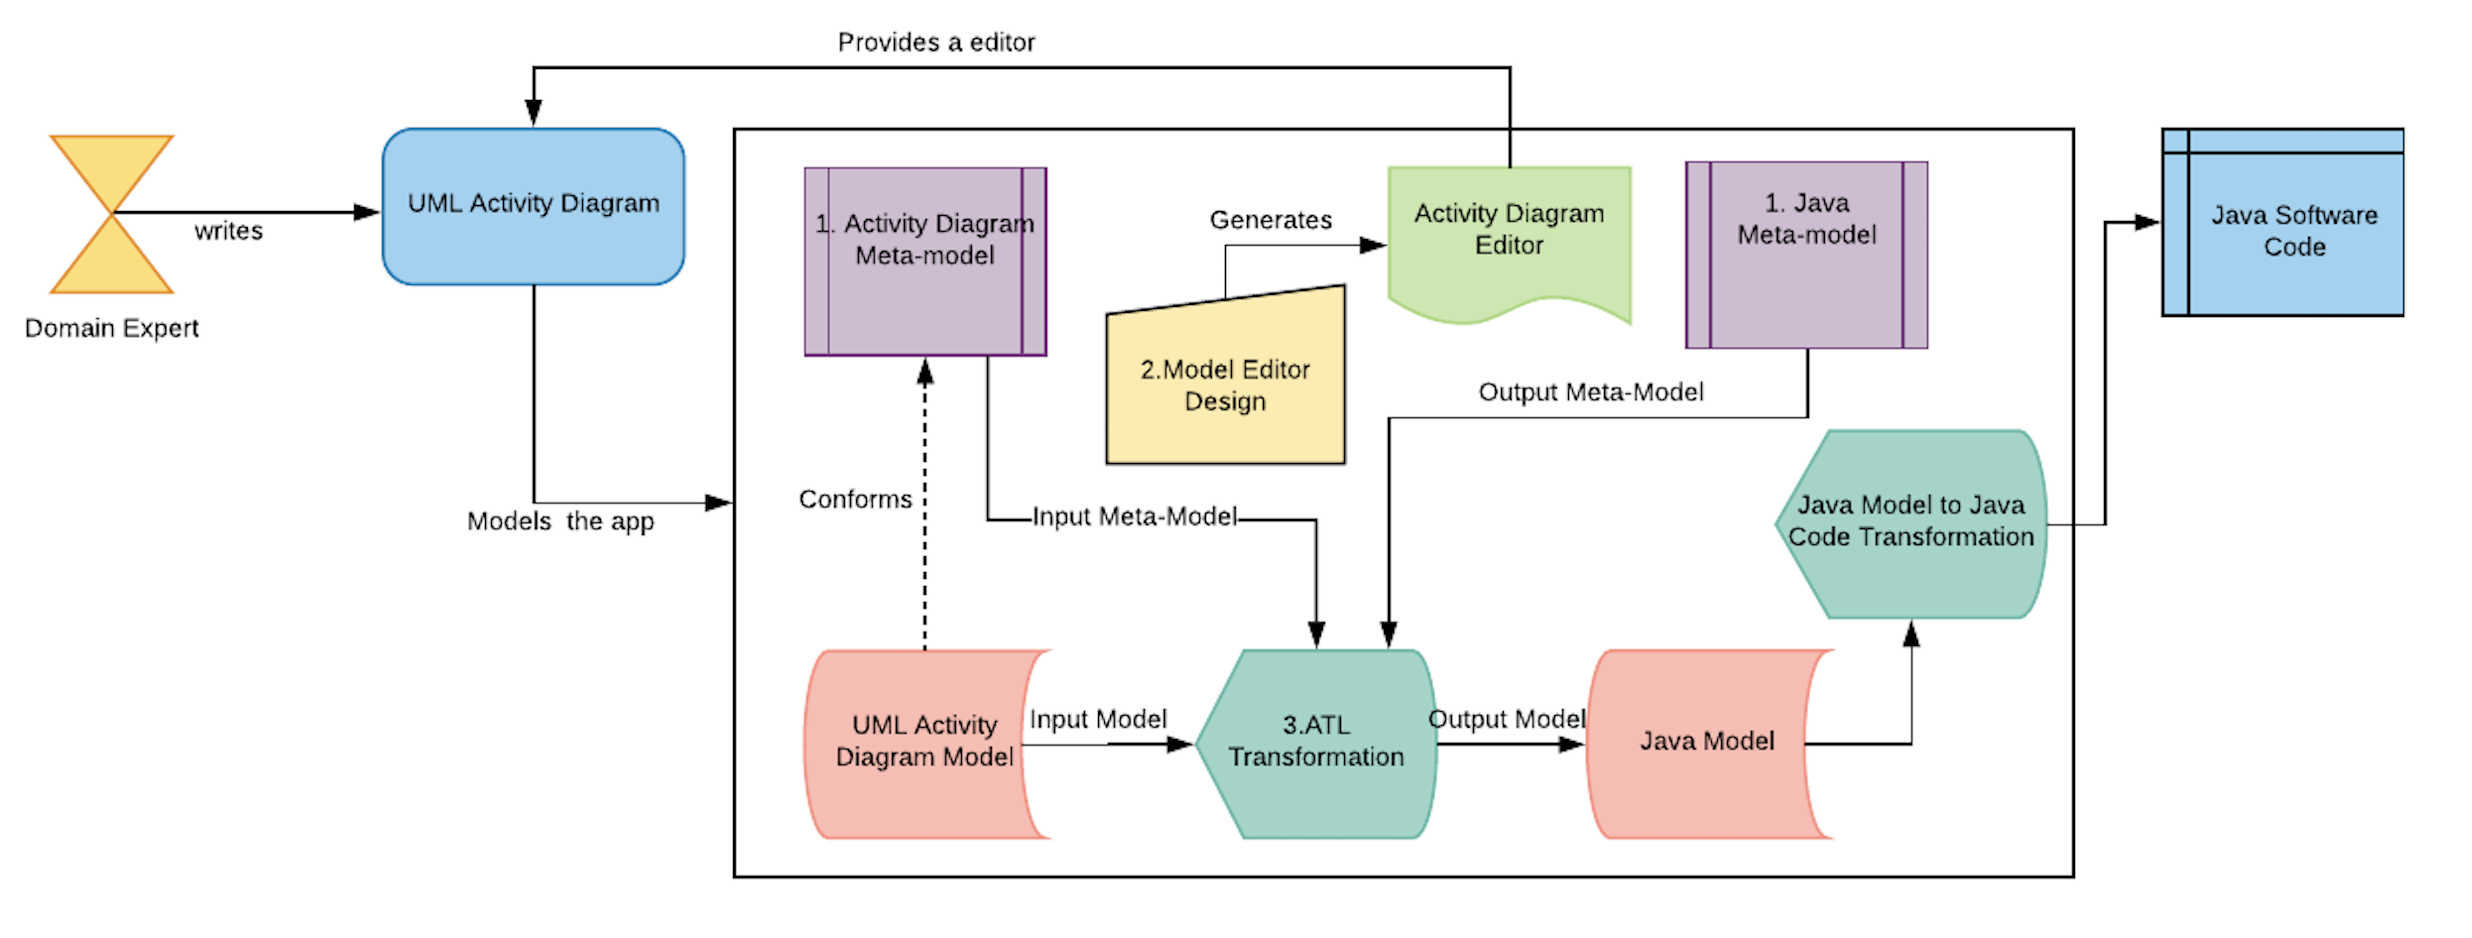
\includegraphics[width=\textwidth]{figs/Architecture_Proposed_Solution}
	\caption{Detailed View of the Architecture}
	\label{figure:overalltool}
\end{figure}

\subsection{Component 1: Meta-Model Design}
\label{Component1}
Component 1 represents the design and development of both the UML Activity Diagram meta-model and the Java meta-model \cite{perera2018thesis}. Meta-models for both Java and UML Activity diagrams are designed using the EMF Framework and Ecore Tools in Eclipse. The Activity Diagram meta-model in shown in Fig.~\ref{figure:ADMetaModel}. 

\begin{figure}[!h]
\centering
	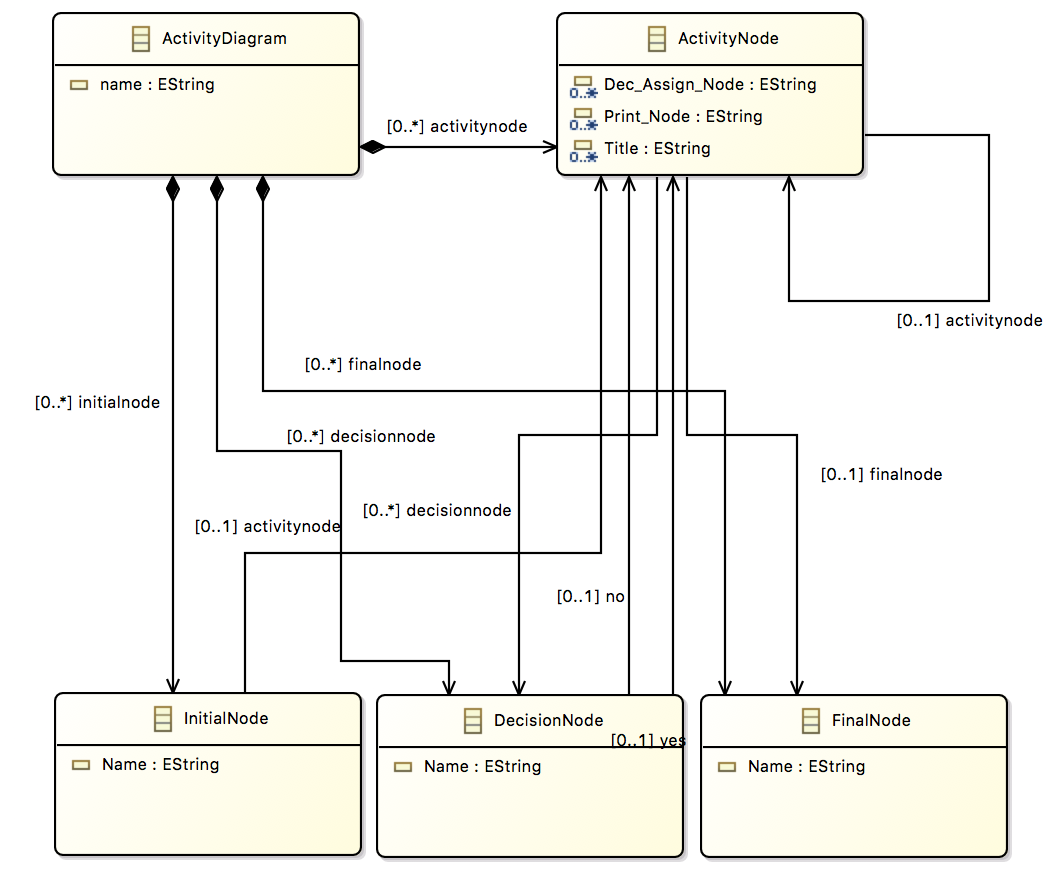
\includegraphics[width=0.8\textwidth]{figs/Activity_Diagram_Meta_Model}
	\caption{Activity Diagram Meta-Model}
	\label{figure:ADMetaModel}
\end{figure}

%The configuration of Figure \ref{figure:ADMetaModel} generates an Activity Diagram Model Instance based on a generic Smart Lighting System. This is shown in the figure below.

\begin{comment}
\begin{figure}[!h]
	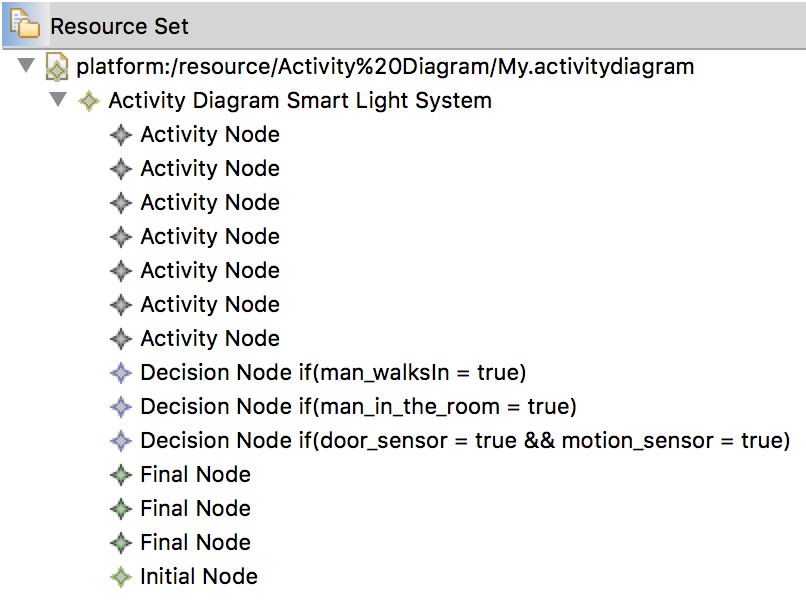
\includegraphics[width=\textwidth]{figs/Activity_Diagram_Model_Instance}
	\caption{Activity Diagram Model Instance (Smart Lighting System)}
	\label{figure:Activity_Diagram_Model_Instance}
\end{figure}
\end{comment}

\subsection{Component 2: Customized Activity Diagram Model Editor}
A customized model editor has been designed with the support of Sirius, an Eclipse plug-in. The model editor consists of a \textit{viewpoint} which supports the connection of the activity diagram meta-model and the model editor. A viewpoint in Sirius provides a set of representations, and in this case, the representation is called "\textbf{\textit{activitydiagram}}" which is synchronized with the activity diagram meta-model. The activation of this viewpoint allows creating and editing of the corresponding activity diagram in the activity diagram model editor \cite{perera2018thesis}. Fig.~\ref{figure:modeleditor} shows a screenshot of the model editor in which a smart lighting system has been modelled.

\begin{figure}[!h]
	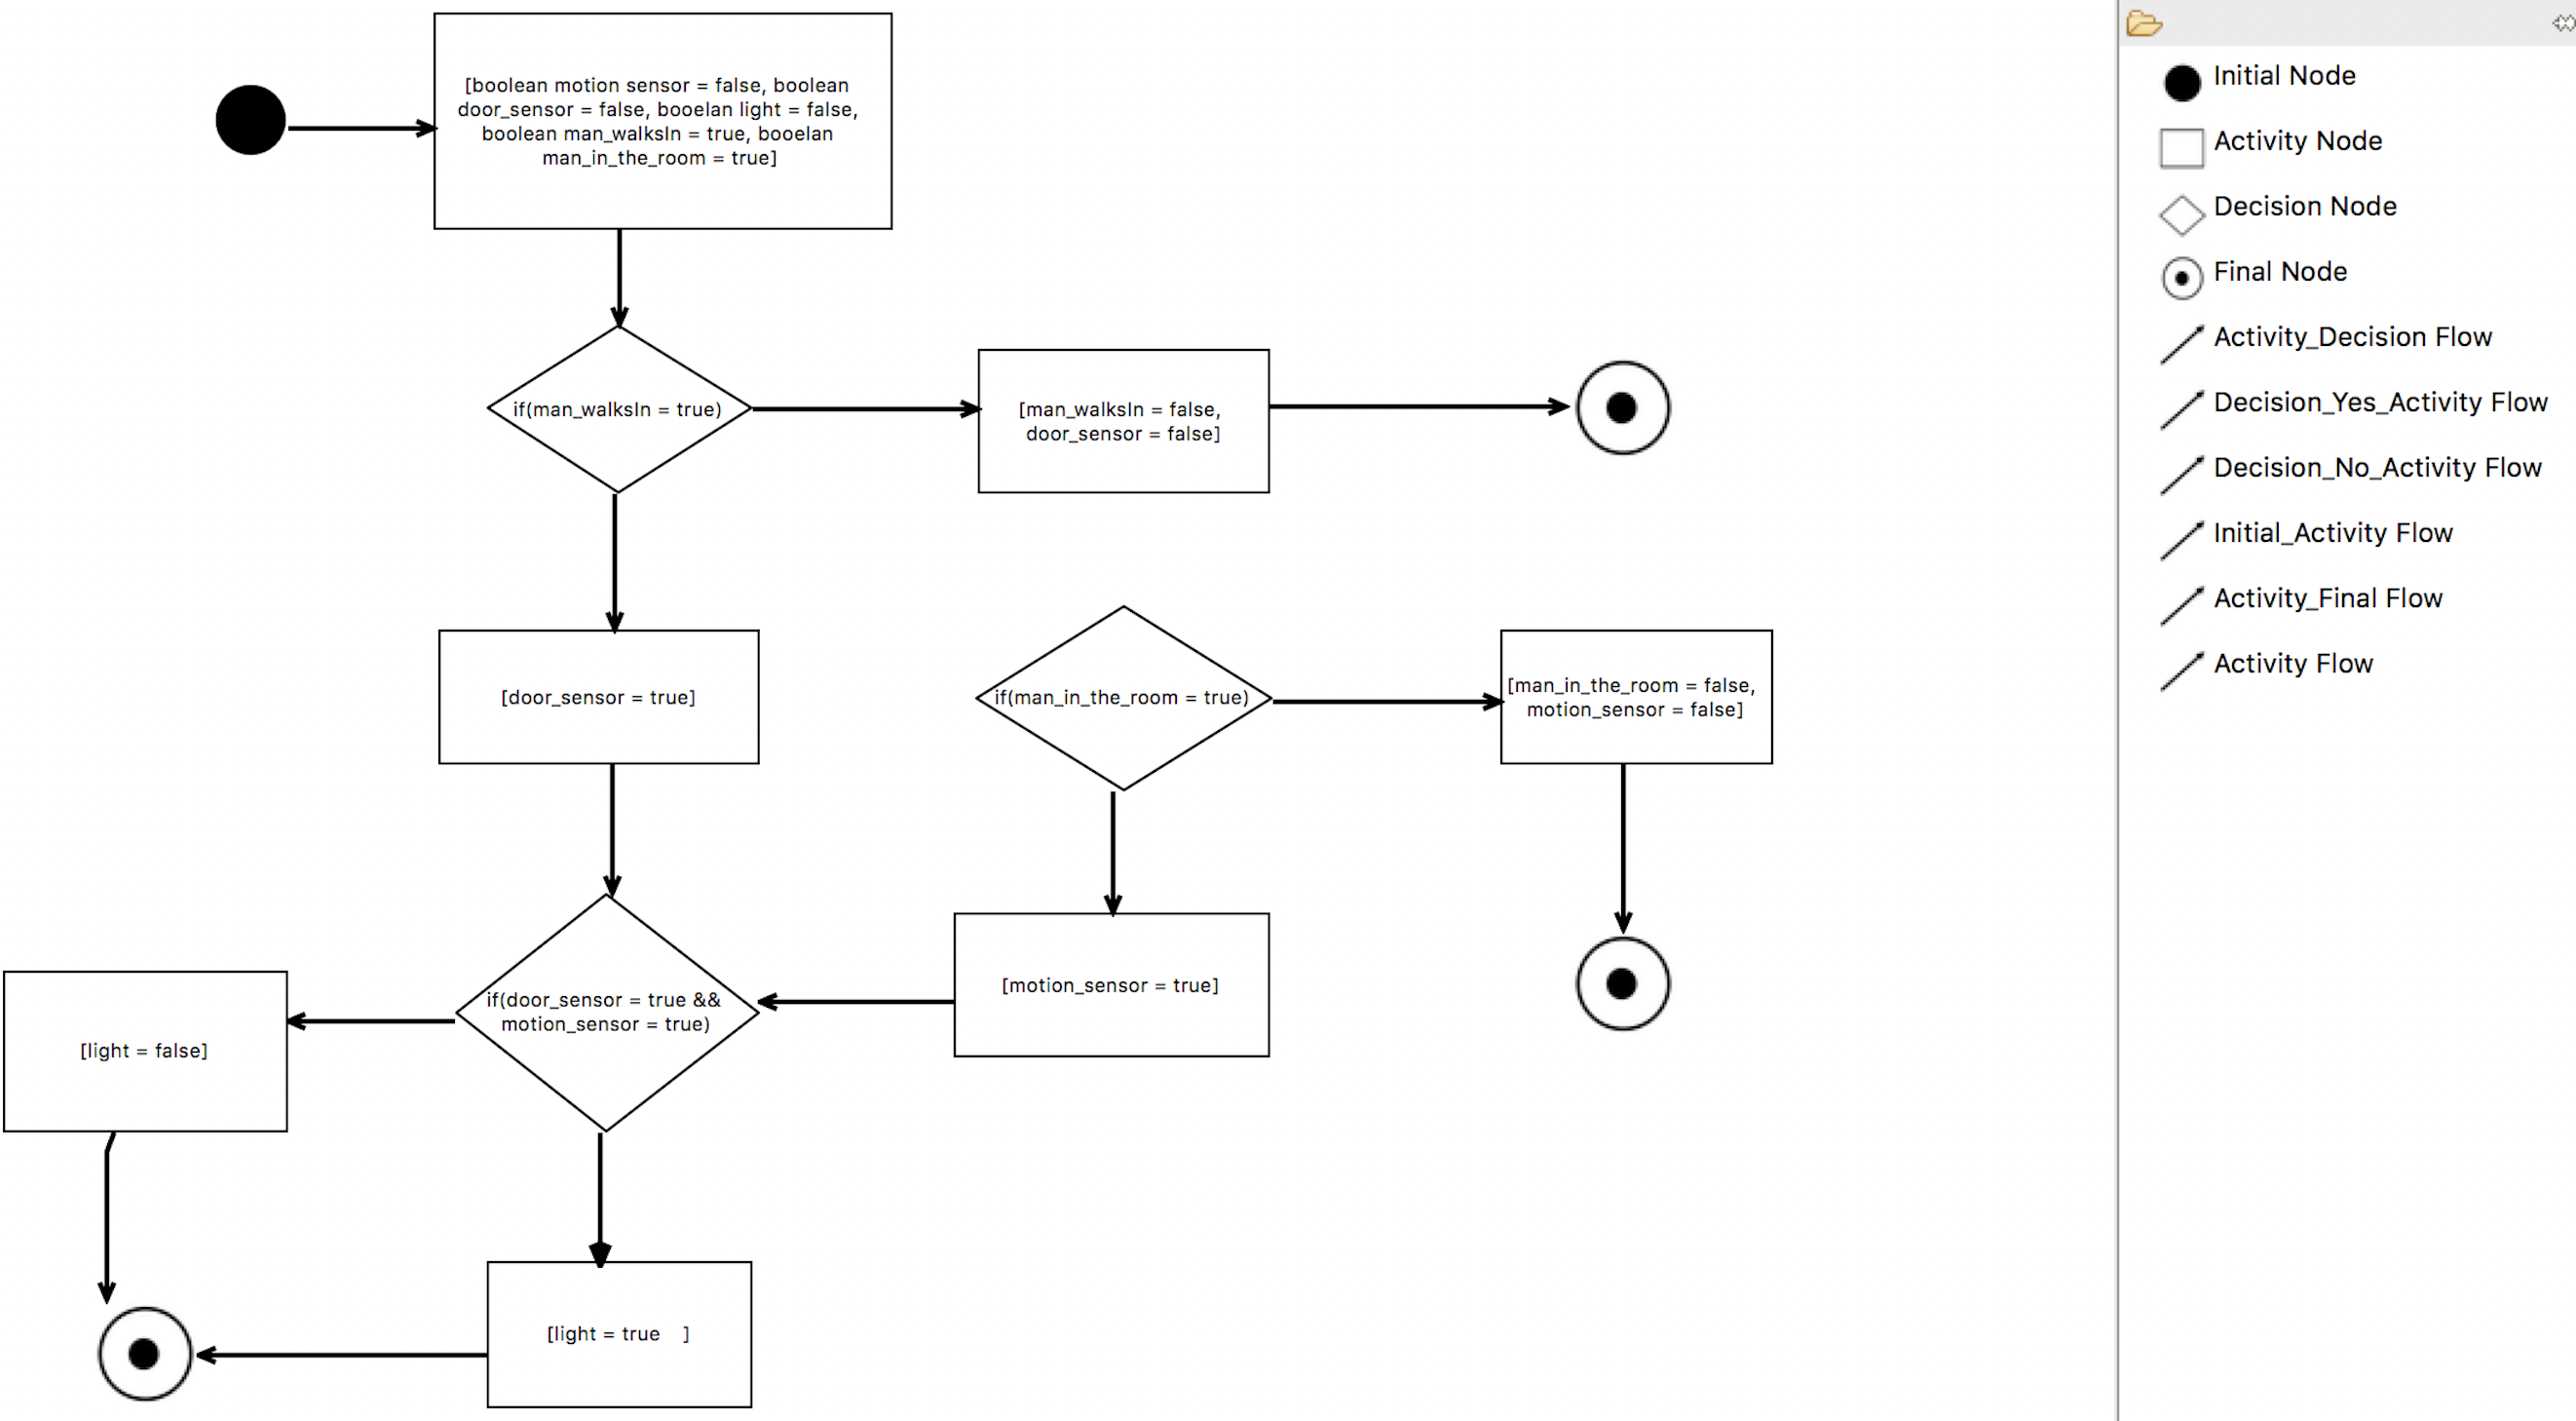
\includegraphics[width=\textwidth]{figs/Activity_Diagram_Model_Editor}
	\caption{Activity Diagram Model Editor depicting a Smart Light System}
	\label{figure:modeleditor}
\end{figure}


\subsection{Component 3: Model-to-Model Transformation}
\label{Component 3: Model-to-Model Transformation}

This technique is used to map the Activity Diagram model to the Java model which eventually supports the generation of software code. ATL is chosen to map and transform models since it is supported by Eclipse which in turn may support the design and development in term of compatibility. The mapping of Activity Diagram Meta-Model and Java Meta-Model with Activity Diagram Model Instance used as the input model (Fig.~\ref{figure:modeleditor}) is shown in Fig.~\ref{figure:ATL_Mapping_Approach}. This configuration process supports the generation of the corresponding Java Model Instance which is later translated into runnable code.

\begin{figure}[!h]
\centering
	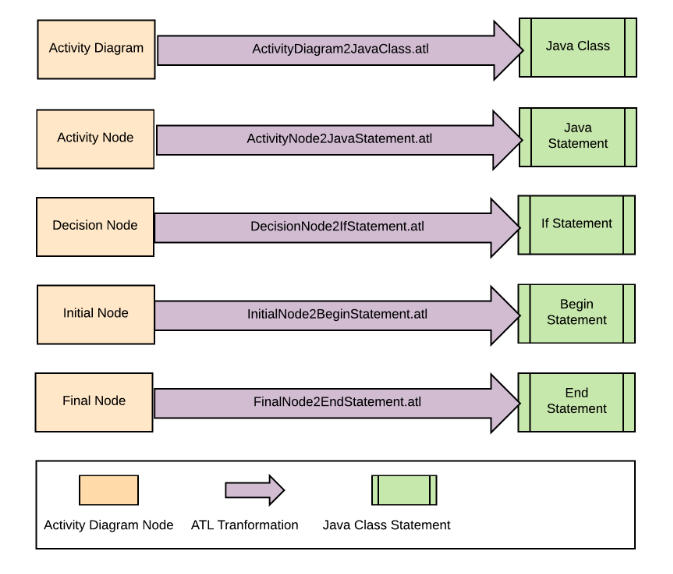
\includegraphics[width=0.6\textwidth]{figs/ATL_Mapping_Approach}
	\caption{ATL Mapping Approach}
	\label{figure:ATL_Mapping_Approach}
\end{figure}



\subsection{Component 4: Model-to-Text Transformation}

The Model-to-Text transformation method is used in the tool to support code generation from the model generated during the mode-to-model transformation. In order to generate Java Code from the model instance which is in XMI format, the file is read using a Java program line by line where each line comprises of a tag name which corresponds with the type of the statements in the code model. Every line is written to a Java file. The Java code generated from the smart lighting system model illustrated in Fig.~\ref{figure:modeleditor} is shown in Fig.~\ref{figure:Generated_Java_Code}.

\begin{figure}[!h]
	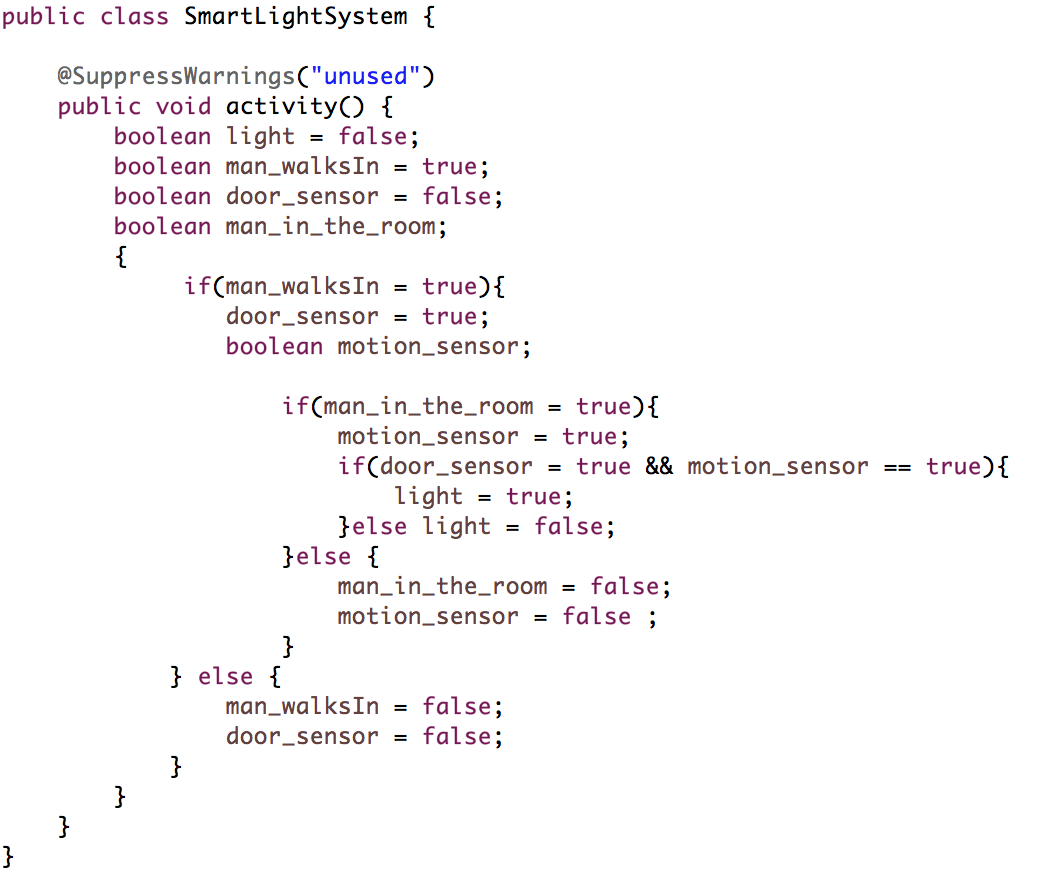
\includegraphics[width=\textwidth]{figs/Generated_Java_Code}
	\caption{Generated Java Code}
	\label{figure:Generated_Java_Code}
\end{figure}



\section{Evaluation and Discussion}
 


This study does not involve the participation of external users, therefore we evaluate the Automatic Translation Tool through four representative smart home apps: Smart Lighting System, Smart Security System. Smart Lock System and Smart Weighting System.
The evaluation criteria for the Automatic Translation Tool are defined based on the quality attribute requirements and primary functional requirements (Sec.~\ref{Architecture Design}). 
To evaluate usability, we count the size of each model, the time taken for creating the model, and the ease at which models can be updated. For other factors, like performance, we look at the size of the generated code and time for compilation. The experimental results for the four case studies are shown in Tab.~\ref{t4}.





\begin{table}[h!]
\scriptsize
\begin{center}
\begin{tabular}{|p{1.7cm}|c|c|c|c|c|p{1.5cm}|c|p{1.5cm}|} \hline
    \textbf{Case Study} & \multicolumn{4}{|c|}{\textbf{Number of Nodes}}&\textbf{Transitions} & \textbf{Modeling Time} & \textbf{Code Size}& \textbf{Compile Time} \\ \hline
    & Activity& Decision& Initial& Final& & & &\\ \hline
    Light System& 7& 3& 3& 1& 14& 12 mins 10 sec &29 lines& 1 min 30 sec\\ \hline
    Security System& 6& 1& 1& 2& 9& 8 mins 32 sec&23 lines &1 min 26 sec\\ \hline
    Door Lock System& 8& 4& 3& 1& 16& 14 mins 12 sec&27 lines& 4 mins 38 sec \\ \hline
    Weighting System& 9& 3& 1& 1& 17&13 mins 45 sec&30 lines& 2 mins 9 sec\\ \hline
\end{tabular} 
\end{center}
\caption{Experimental Data to Model Smart Home Systems}
\label{t4}
\end{table}


 
Overall, the times taken to model the smart home systems are relatively similar. However, usability was negatively affected by the installation time for the software, due to the need for several Eclipse plugins. This weakness can be addressed through the development of an integrated installer for the tool in the future.
The time taken for updating every smart home app was remarkably small, which is attributed to the similarity of activity diagrams to flowcharts. 

However, compilation times for each of the study as shown in \ref{t4} are relatively high. The Smart Security System, which has the smallest size, takes the shortest time to compile. The long compile times come from the manual effort that the tool currently requires in the intermediate stages of the code generation process. For instance, intermediate files generated after a model transformation have to be manually pasted into a different folder for the next phase. These are purely mechanical steps that can be automated easily in the future, and we are already working on these. 






\section{Conclusions and Future Works}

We propose an Automatic Translation Tool that takes in UML Activity Diagrams and generates Java code for smart home apps. Starting with a systematic literature review, we identified the useful features of a usable app design model. We also found that current design models do not completely support these factors. Following a qualitative review of UML diagrams, we identify UML Activity Diagrams as the best available option for modelling smart home apps. We then focussed on architecting a solution for generating executable code from UML Activity Diagrams. We identified primary architectural drivers, which included usability and modularity as the prime quality attributes. We then presented both the logical and process views of this architecture, built using architectural patterns and tactics that supported the architectural drivers. Then, we developed the automatic translation tool which carries out a number of model transformations to convert visual designs in Java code. These visual designs are created in a model editor that we also developed. We evaluated the tool through four representative case studies, and observed that it successfully achieves the primary architectural drivers, albeit it does need some further development to completely automate the compilation process. 

Other future directions include adapting UML Activity Diagrams for specific domains such as primary health such that domain experts can build app models using vocabulary that they are more familiar with. 
In terms of the Java code generation, code is generated for the respective activities modeled in the Activity Diagram Model Editor, therefore code generated from the tool only defines the behavior of an object and does not include the structure of the code such as class and method declarations. Currently, each design is contained within its own class. For larger problems, the tool should allow the user to provide some structural information as well. 
Hence, a more specific modeling language  that supports both behavioral and structural aspects of a system could be chosen. 




\bibliographystyle{splncs03}
\bibliography{references}



\end{document}
